\chapter{Guía de usuario}
\label{chap:guía de usuario}

\section{Interfaz gráfica}

Una interfaz gráfica de usuario (GUI) presenta un mecanismo amigable al usuario para interactuar con una aplicación. Una GUI proporciona a una aplicación una ``apariencia visual'' única. Al proporcionar distintas aplicaciones en las que los componentes de la interfaz de usuario sean consistentes e intuitivos, los usuarios pueden familiarizarse en cierto modo con una aplicación, de manera que pueden aprender a utilizarla en menor tiempo y con mayor productividad.\\

Las GUIs se crean a partir de componentes de la GUI. A éstos se les conoce también como controladores o widgets (accesorios de ventana) en otros lenguajes. Un componente de la GUI es un objeto con el cual interactúa el usuario mediante el ratón, el teclado u otra forma de entrada, como el reconocimiento de voz.\\

\section{Componentes GUI en java}

En java existen realmente dos conjuntos de componentes de GUI. Antes de introducir a Swing en Java SE 1.2, las GUIs de Java se creaban a partir de componentes del \textbf{Abstract Window Toolkit (AWT}) en el paquete \textbf{java.awt}. Cuando una aplicación de Java con una GUI del AWT se ejecuta en distintas plataformas, los componentes de la GUI de la aplicación se muestran de manera distinta en cada plataforma. Consideremos una aplicación que muestra un objeto de tipo \emph{Button} (paquete \emph{java.awt}). En una computadora que ejecuta el sistema operativo Microsoft Windows, el objeto \emph{Button} tendrá la misma apariencia que los botones en las demás aplicaciones Windows. De manera similar, en una computadora que ejecuta el sistema operativo Apple Mac OS X, el objeto \emph{Button} tendrá la misma apariencia visual que los botones en las demás aplicaciones Macintosh. Algunas veces, la forma en la que un usuario puede interactuar con un componente específico del AWT difiere entre una plataforma y otra.\\

En conjunto, a la apariencia y la forma en la que interactúa el usuario con la aplicación se les denomina la \textbf{apariencia visual}. Los componentes de GUI de Swing nos permiten especificar una apariencia visual uniforme para una aplicación a través de todas las plataformas, o para usar la apariencia visual personalizada de cada plataforma. Incluso, hasta una aplicación puede modificar la apariencia visual durante la ejecución, para permitir a los usuarios elegir su propia apariencia visual preferida.\\

\section{Introducción}

En este documento se describirá los objetivos e información clara y concisa de cómo utilizar la Suite de Teoría Algorítmica de grafos: Graphvisualx.\\

La Suite de Teoría Algorítmica de grafos: Graphvisualx ha sido creado por Moisés Gautier Gómez para el proyecto de fin de carrera de la titulación de ingeniería informática técnica de sistemas de la universidad de Cádiz. El objetivo es facilitar en la compresión de los estudiantes de la materia de grafos en la resolución de ejemplos de los mismos empleando los algoritmos más conocidos y que usualmente se emplean en el entorno académico.\\

Es de mucha importancia consultar esta guía antes y/o durante la utilización de la Suite, ya que lo guiará paso a paso en el manejo de las funciones de ella. La resolución recomendada para la aplicación debe ser superior o igual a 1024 x 768 (Estándar XGA). \\

Con el fin de facilitar la comprensión de la guía, se incluye gráficos explicativos. Los iconos de la aplicación se han obtenido de la página web \url{http://www.iconfinder.com}. \\

\section{Objetivo de esta guía}

El objetivo primordial de esta guía es ayudar y guiar al usuario a utilizar la Suite de Teoría Algorítmica de grafos: Graphvisualx obteniendo la información adecuada de los algoritmos para despejar todas las dudas existentes y comprende:

\begin{itemize}
\item Guía para acceder a la Suite.
\item Conocer como utilizar la Suite, mediante una descripción detallada e ilustrada de opciones.
\item Conocer el alcance de todos los algoritmos por medio de una explicación detallada de ellos e ilustrada en el manual de algoritmos que se adjuntará en la guía y que también será accesible desde la Suite.
\end{itemize}

\section{Dirigido a}

Esta guía esta dirigida al usuario final de la Suite que utilicen dicho recurso como complemento al material docente de asignaturas de la titulación así como laboratorio de pruebas de algoritmos sobre grafos de ejemplo.

\section{Convenciones y estándares a utilizar}

Entre las convenciones y estándares a utilizar tenemos las siguientes:

\subsection{Convenciones del uso del ratón}

\begin{table}[H]
\begin{tabular}{|p{2cm}|p{3cm}|p{5cm}|p{5cm}|}
\hline
\centering{Término} & \centering{Situación} & \centering{Elemento aplicación} & \qquad \quad Significado \\
\hline
\centering{
\includegraphics[scale=.6]{./imagenes_documentacion/mouse.png}} & - & Sobre cualquier botón & Apertura del menú o acción designado para tal botón. \\
\hline
\multicolumn{4}{|c|}{Modo edición grafo} \\
\hline
\centering{
\includegraphics[scale=.6]{./imagenes_documentacion/mouse_left.png}} & Sobre lienzo de trabajo & Modo crear nodos sobre el lienzo (Botón crear nodo previamente pulsado). & Crea un nodo en el espacio designado para ello. \\
\hline
\centering{
\includegraphics[scale=.6]{./imagenes_documentacion/mouse_right.png}} & Sobre nodo creado en el lienzo de trabajo & Modo crear nodo sobre el lienzo (Botón crear nodo previamente pulsado). & Elimina el nodo creado anteriormente en el nodo. Se reorganiza la numeración del etiquetado de nodos si fuera necesario. \\
\hline
\centering{
\includegraphics[scale=.6]{./imagenes_documentacion/mouse_left.png}} & Sobre un nodo creado y arrastrar el cursor a otro nodo creado. Soltar inmediatamente. & Modo crear arista sobre el lienzo (Botón crear arista previamente pulsado). & Crea una arista de adyacencia (si es dirigido el grafo con la flecha de finalización apuntando hacia el nodo destino) sobre el nodo origen hacia el nodo destino. \\
\hline
\centering{
\includegraphics[scale=.6]{./imagenes_documentacion/mouse_right.png}} & Sobre una arista creada previamente (sobre la etiqueta de ponderación de la misma). & Modo crear arista sobre el lienzo (Botón crear arista previamente pulsado). & Da la opción de modificar el coste/ponderación de la arista o de eliminarla. \\
\hline
\end{tabular}
\end{table}
\newpage
\begin{table}[H]
\begin{tabular}{|p{2cm}|p{3cm}|p{5cm}|p{5cm}|}
\hline
\centering{
\includegraphics[scale=.6]{./imagenes_documentacion/mouse_left.png}} & - & Modo eliminar contenido lienzo. & Elimina todos los elementos contenidos en el lienzo de trabajo. \\
\hline
\centering{
\includegraphics[scale=.6]{./imagenes_documentacion/mouse_both.png}} & Sobre un nodo creado en el lienzo de trabajo & Modo mover nodos (Botón mover nodos previamente pulsado) & Permite cambiar de posición el nodo dentro de lienzo según las preferencias del usuario. \\
\hline
\centering{
\includegraphics[scale=.6]{./imagenes_documentacion/mouse_left.png}} & - & Modo aceptar grafo & Concluye la edición del lienzo de trabajo para la creación de un grafo. \\
\hline
\end{tabular}
\end{table}

\subsection{Convenciones del uso del teclado}

\begin{table}[H]
\begin{center}
\begin{tabular}{|p{6cm}|p{8cm}|}
\hline
\centering{Tecla} & \qquad \quad Significado \\
\hline

\includegraphics[width=5.5cm]{./imagenes_documentacion/key_ctrl_g.png} & \vspace*{-.8in}{Guardar el grafo inicial. Abre un menú emergente en donde te permite guardar un fichero en formato texto plano en el sistema con el nombre que se desee. No hay que escribir explícitamente la extensión al definir el nombre del fichero, es decir, con escribir ``ejemplo'' el sistema asigna la extensión al nombre inmediatamente.} \\
\hline

\includegraphics[width=5.5cm]{./imagenes_documentacion/key_ctrl_x.png} & \vspace*{-.8in}{Salir de la Suite. Cierra la Suite y para volver a acceder a ella se tendrá que hacer doble clic sobre el lanzador.} \\
\hline
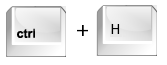
\includegraphics[width=5.5cm]{./imagenes_documentacion/key_ctrl_h.png} & \vspace*{-.8in}{Guía del usuario. Se abre una nueva ventana en donde vendrá definida la guía del usuario para cualquier duda sobre el uso de Graphvisualx.} \\
\hline

\includegraphics[width=5.5cm]{./imagenes_documentacion/key_ctrl_m.png} & \vspace*{-.8in}{Manual de los algoritmos y conceptos relacionados con la teoría algorítmica de grafos. Se abre una nueva ventana en donde vendrá definido un documento en formato pdf con los contenidos teóricos necesarios en caso de duda.} \\
\hline
\end{tabular}
\end{center}
\end{table}
\newpage
\begin{table}[H]
\begin{center}
\begin{tabular}{|p{6cm}|p{8cm}|}
\hline
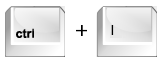
\includegraphics[width=5.5cm]{./imagenes_documentacion/key_ctrl_i.png} & \vspace*{-.8in}{Sobre Graphvisualx. Se abre una nueva ventana donde viene información sobre el autor de Graphvisualx y demás.} \\
\hline
\end{tabular}
\end{center}
\end{table}

\section{Ingreso al sistema}

Una vez descargada la aplicación y colocada en el directorio deseado hacemos doble clic sobre ella para ejecutar la Suite. Sino se produciese ningún evento probar con la siguiente opción:
\begin{figure}[H]
\hspace*{-.75in}{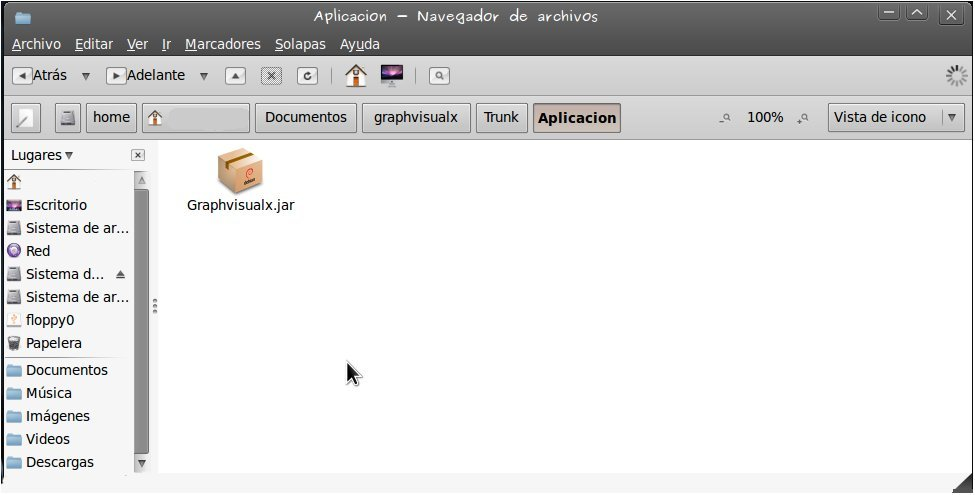
\includegraphics[width=20cm]{./imagenes_documentacion/captura_1.jpeg}}
\caption{Directorio de trabajo donde se encuentra el fichero .jar ejecutable de la Suite.}
\end{figure}
\newpage
\begin{figure}[H]
\hspace*{.5in}{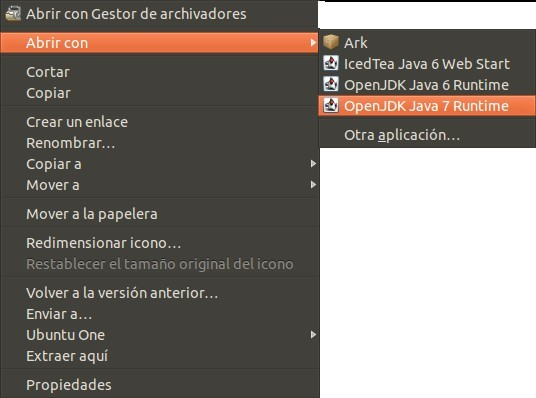
\includegraphics[width=13cm]{./imagenes_documentacion/desplegable_menu_abrir_jar.jpeg}}
\caption{Menú desplegable al pulsar botón derecho sobre el ejecutable .jar y selección de programa.}
\end{figure}

\subsection{Como acceder a la suite}
\label{cap:Acceder}

Si no se dispusiese de máquina virtual java en el sistema se deberá instalar a través de línea de comandos en el terminal de GNU/Linux.
Para ello primeramente hay que escribir \url{http://www.java.com/es/download/help/linux_install.xml} en nuestro navegador favorito para ir a la página web de java, en donde se nos explica el método de instalación a seguir. Sea pues:
\newpage
\begin{figure}[H]
\hspace*{-.8in}{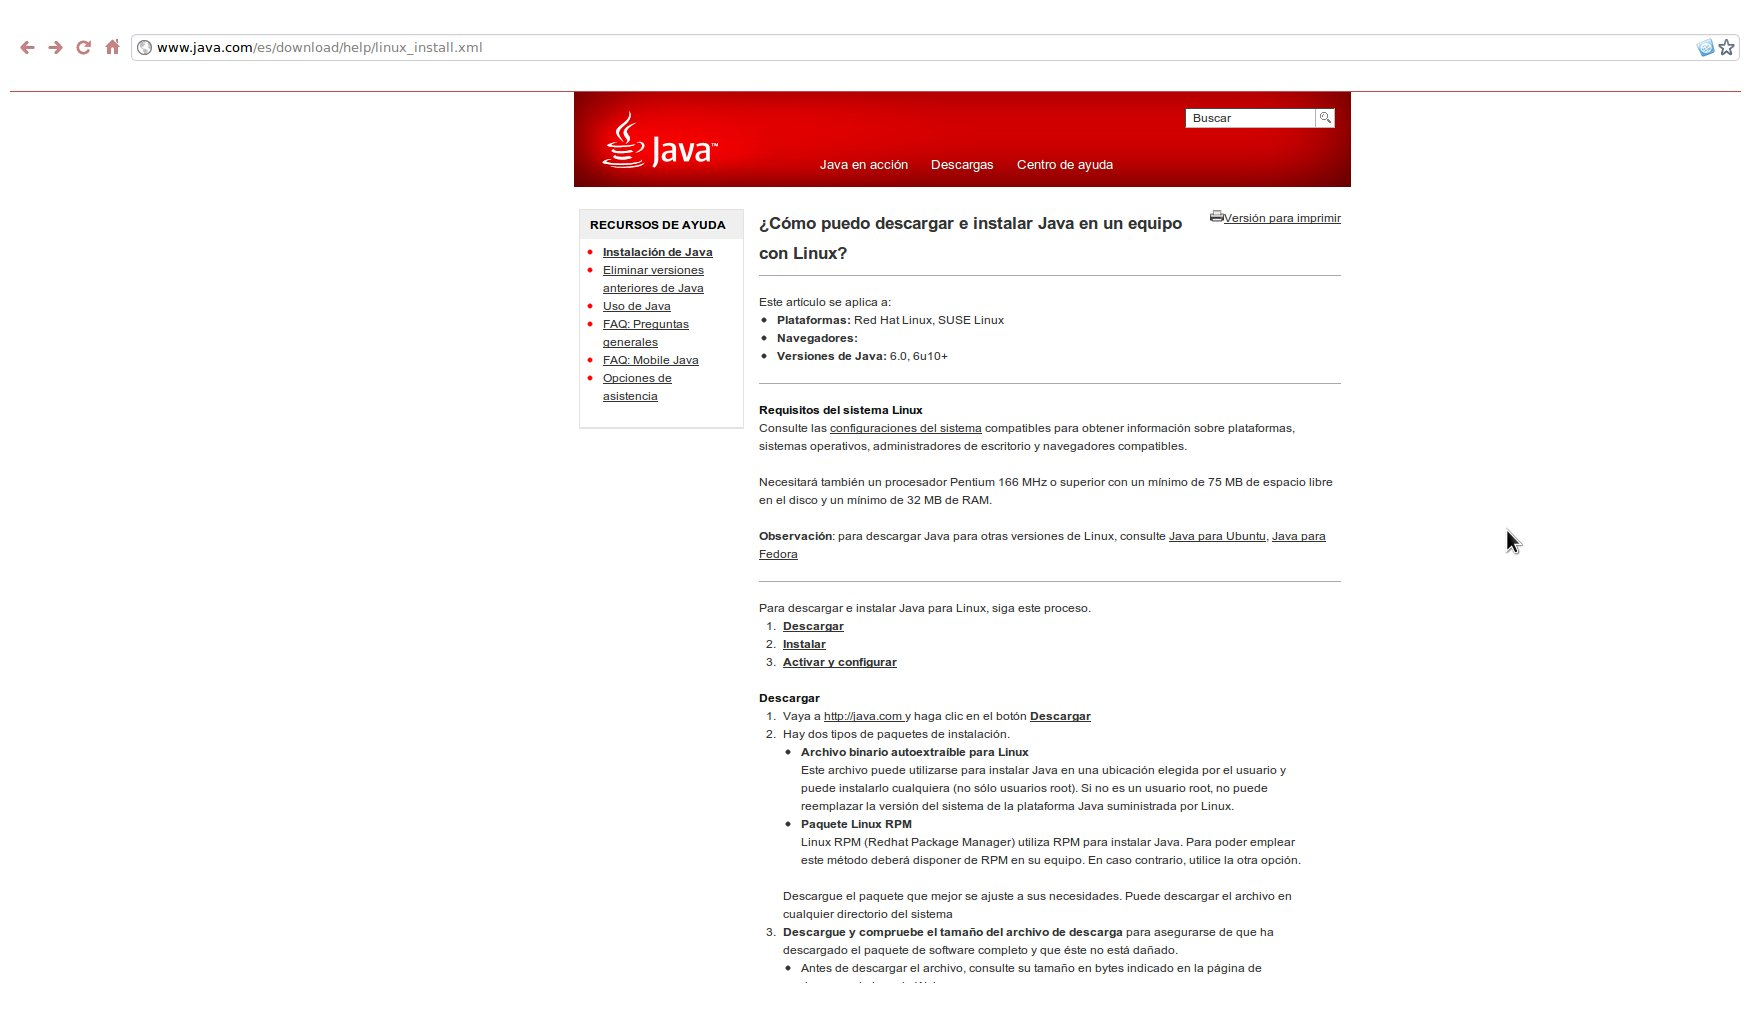
\includegraphics[width=20cm]{./imagenes_documentacion/captura_2.jpeg}}
\caption{Página web de Java donde se explican los pasos para la instalación del software Java en nuestro sistema GNU/Linux.}
\end{figure}

\begin{figure}[H]
\hspace*{-.8in}{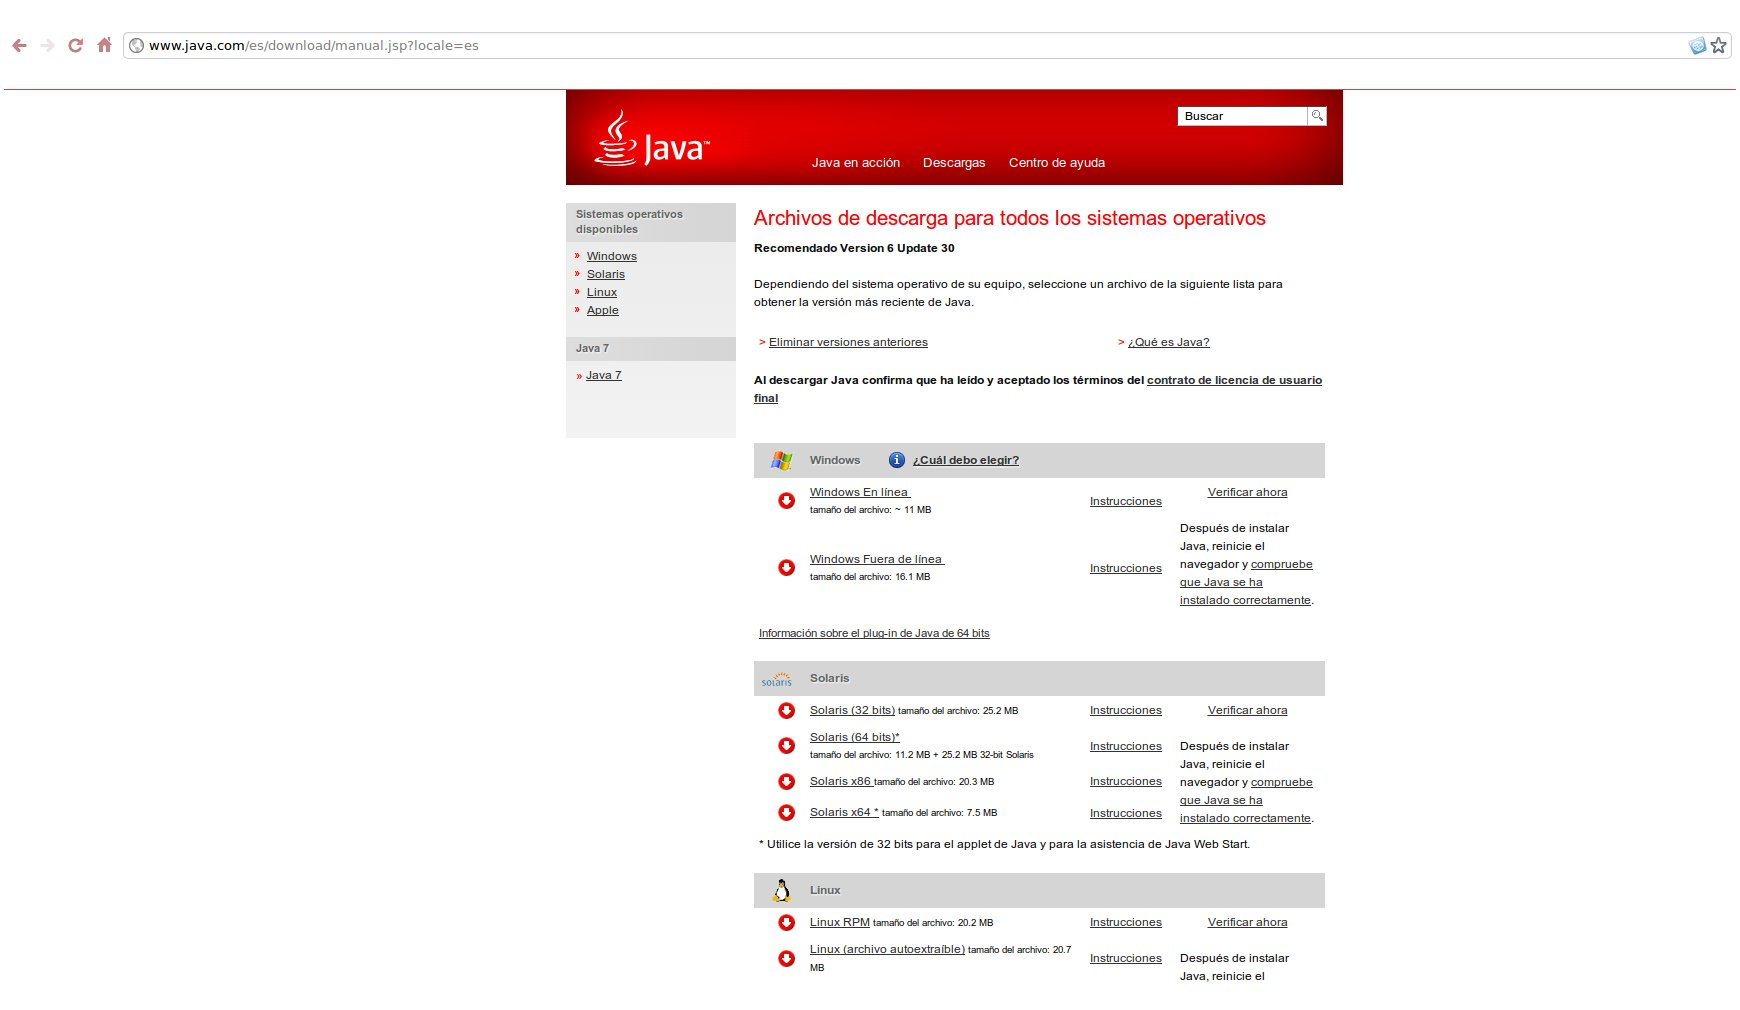
\includegraphics[width=20cm]{./imagenes_documentacion/captura_3.jpeg}}
\caption{Página web donde se encuentran los ficheros descargables según sistema operativo \url{http://www.java.com/es/download/manual.jsp?locale=es}.}
\end{figure}

\begin{figure}[H]
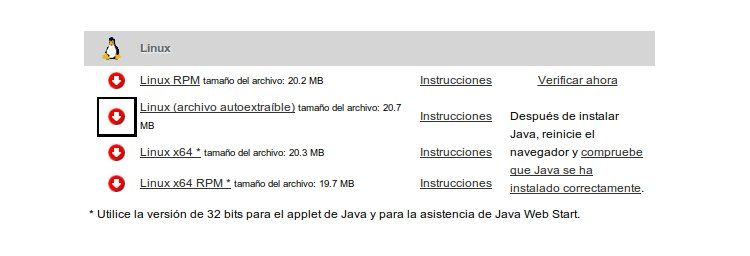
\includegraphics[width=15cm]{./imagenes_documentacion/captura_4.jpeg}
\caption{Sección de la página web de la figura 7.4 en donde se especifica para el sistema operativo GNU/Linux.}
\end{figure}

Si se desea la descarga del archivo en formato ``.rpm'' se deberá poner en la línea de comandos para su instalación el comando:\\

\begin{center} \emph{rpm -Uvh nombre\_paquete.rpm}\\ \end{center}

Si por el contrario se descarga el fichero en formato autoextraible será necesario escribir el siguiente comando en la línea de comandos:\\

\begin{center} \emph{sh nombre\_paquete.bin}\\ \end{center}

Además de todo ello se deberá tener instalado también el jdk de java para poder visualizar la aplicación perfectamente en nuestro sistema. Para ello tenemos que teclear en línea de comandos:\\
\begin{center} \emph{sudo apt-get install openjdk-jre} \\ \end{center}

\subsection{Problemas con los permisos de la aplicación}

Hay veces en las que la generación de documentos en un sistema GNU/Linux sigue las directrices de la función/orden umask que establece los permisos por defecto de todos los nuevos ficheros en el sistema de archivos. Según sea el caso nuestro sistema puede no ser capaz de realizar la ejecución de la aplicación por la falta de alguno de los permisos necesarios.\\

\begin{figure}[H]
\begin{center}
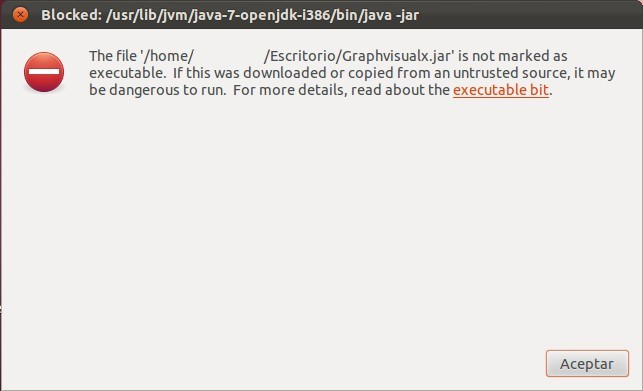
\includegraphics[width=16cm]{./imagenes_documentacion/captura_error_ejecucion_jar.jpeg}
\caption{Mensaje de error al no tener habilitados los permisos de ejecución la aplicación.}
\end{center}
\end{figure}

Para ello será necesario posicionarse en el directorio donde se encuentre la aplicación, a través de una terminal/consola en nuestro sistema GNU/Linux favorito, y teclear el siguiente comando:\\

\begin{center} \emph{chmod +x Graphvisualx.jar} \\ \end{center}

\subsection{Paquetes adicionales para distribuciones GNU/Linux}

Para la generación de los ficheros en formato imagen de los grafos es necesario instalar en su sistema el paquete graphviz, que es un software de código abierto empleado en la visualización de grafos. Sin este software el fichero generado por el módulo de la aplicación (Graphviz.java) en formato .dot no puede ser interpretado por el sistema para su posterior transformación a imagen visual.\\

Nos dirigimos a una terminal en donde debemos introducir el siguiente comando:

\begin{center} \emph{sudo apt-get install graphviz} \\ \end{center}

Por motivos de eficiencia el algoritmo de compresión de imágenes será .png dado que es muy práctico y extendido para imágenes que no requieran de un alto contenido de detalles, conservando todos los colores posibles.

\section{Operaciones de la suite}
\subsection{Archivo}

Icono representativo: 
\includegraphics[scale=.7]{./imagenes_documentacion/archivo.png} \\

Dentro de este apartado se definirán los items del menú de archivo. En él se encuentran cuatro posibles operaciones a realizar por el usuario según haya o no:
\begin{itemize}
\item Creado un grafo mediante su edición o cargado en el sistema.
\item Procesado dicho grafo mediante algún algoritmo.
\item En caso contrario, no haber realizado ninguna operación con el sistema.
\end{itemize}

Para el caso de que el usuario haya simplemente cargado o editado un grafo en el sistema, tendrá las siguientes operaciones disponibles (o items) del menú archivo.

\begin{itemize}
\item Guardar grafo inicial (Atajo de teclado Ctrl+g). \quad 
\includegraphics[scale=.9]{./imagenes_documentacion/guardar.png} 
\item Guardar grafo como imagen. \quad 
\includegraphics[scale=.15]{./imagenes_documentacion/guardar_imagen.png}
\item Salir (Atajo de teclado Ctrl+x). \quad 
\includegraphics[scale=.9]{./imagenes_documentacion/exit.png}
\end{itemize}

Cuando el usuario haya procedo un grafo, previamente definido en el sistema, con uno de los algoritmos posibles tendrá las siguientes operaciones disponibles (o items) del menú archivo.

\begin{itemize}
\item Guardar grafo inicial (Atajo de teclado Ctrl+g). \quad 
\includegraphics[scale=.9]{./imagenes_documentacion/guardar.png} 
\item Guardar grafo como imagen. \quad 
\includegraphics[scale=.15]{./imagenes_documentacion/guardar_imagen.png}
\item Guardar grafo resultado como imagen. \quad 
\includegraphics[scale=.15]{./imagenes_documentacion/guardar_imagen.png}
\item Salir (Atajo de teclado Ctrl+x). \quad 
\includegraphics[scale=.9]{./imagenes_documentacion/exit.png}
\end{itemize}

En caso contrario de no haber realizado ninguna operación con el sistema, tendrá las siguientes operaciones disponibles (o items) del menú archivo.

\begin{itemize}
\item Salir (Atajo de teclado Ctrl+x). \quad 
\includegraphics[scale=.9]{./imagenes_documentacion/exit.png}
\end{itemize}

Guardar grafo inicial permite al usuario, una vez haya realizado la edición o creación de un nuevo grafo en el sistema, guardar la estructura interna del grafo en un fichero en formato de texto plano en su sistema de ficheros para posteriormente simplemente cargar dicho fichero sin necesidad de editar de nuevo todo su contenido. No es necesario establecer la extensión de ``.txt'' al nombre del archivo, ya que automáticamente el sistema dota de tal extensión al nombre adjunto. Su atajo de teclado es: Ctrl+G. \\

\begin{figure}[H]
\begin{center}
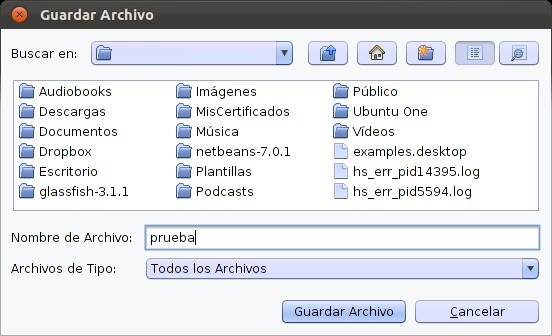
\includegraphics[width=13cm]{./imagenes_documentacion/imagen_guardar_archivo.jpeg}
\caption{Listado de directorios donde se puede seleccionar el destino del archivo.}
\end{center}
\end{figure}

Guardar grafo como imagen permite al usuario, una vez haya realizado la edición o creación de un nuevo grafo en el sistema, guardar la estructura visual del grafo en un fichero en formato imagen (png) en su sistema de ficheros para posteriormente usarla como material adicional de un trabajo o simplemente para almacenar de una manera visual dicho contenido en vez del fichero de texto plano. Esta opción no permite guardar el grafo para posteriores cargas en el sistema, ya que simplemente se limita a crear una representación con graphviz del contenido del grafo. En ningún momento se almacena la estructura del mismo adjunta a la imagen. Para ello es necesario usar la opción anterior de ``Guardar grafo inicial''.\\

\begin{figure}[H]
\begin{center}
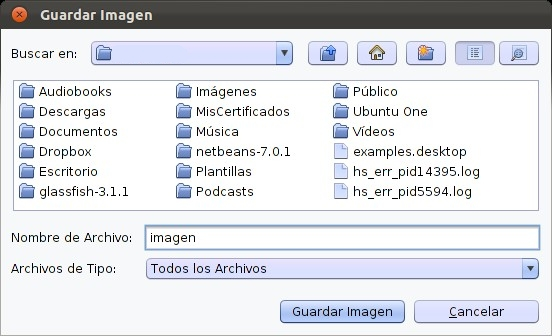
\includegraphics[width=13cm]{./imagenes_documentacion/imagen_guardar_imagen.jpeg}
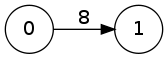
\includegraphics[width=3cm]{./imagenes_documentacion/grafo.png}
\caption{Listado de directorios donde se puede seleccionar el destino del archivo e imagen resultante.}
\end{center}
\end{figure}

Guardar grafo resultado como imagen permite al usuario, una vez haya realizado algún procesamiento sobre un grafo del sistema, guardar la estructura visual del grafo resultado del procesamiento en un fichero en formato imagen (png) en su sistema de ficheros para posteriormente usarla como material adicional de un trabajo o simplemente para almacenar de una manera visual dicho resultado. \\

Salir, según su nombre indica, permite al usuario abandonar la aplicación. Su atajo de teclado es: Ctrl+x. \\
\subsection{Ayuda}

Icono representativo: 
\includegraphics[scale=.2]{./imagenes_documentacion/ayuda.png} \\

Dentro de este apartado se definirán los items del menú de ayuda. En él se encuentran tres posibles operaciones de consulta para el usuario.
\begin{itemize}
\item Guía de uso (Atajo de teclado Ctrl+h). \quad 
\includegraphics[scale=.95]{./imagenes_documentacion/guide.png}
\item Algoritmos y conceptos (Atajo de teclado Ctrl+m). \quad 
\includegraphics[scale=.9]{./imagenes_documentacion/manual.png}
\item Sobre Graphvisualx (Atajo de teclado Ctrl+I). \quad 
\includegraphics[scale=.9]{./imagenes_documentacion/about.png}
\end{itemize}

La guía de uso servirá para solventar las dudas de uso de la aplicación. En ella se hará un recorrido por todas las funcionalidades de la suite, así como los posibles usos que tiene cada componente de la misma. Su atajo de teclado es: Ctrl+h. \\

En el menú de algoritmos y conceptos se describe paso a paso, para los casos descritos, los conceptos y algoritmos usados para la Suite informática de Teoría Algorítmica de Grafos. Se hará uso de trazas en ciertos casos y su representación en formato código java en la que se basa la suite. Su atajo de teclado es: Ctrl+m. \\

\begin{figure}[H]
\begin{center}
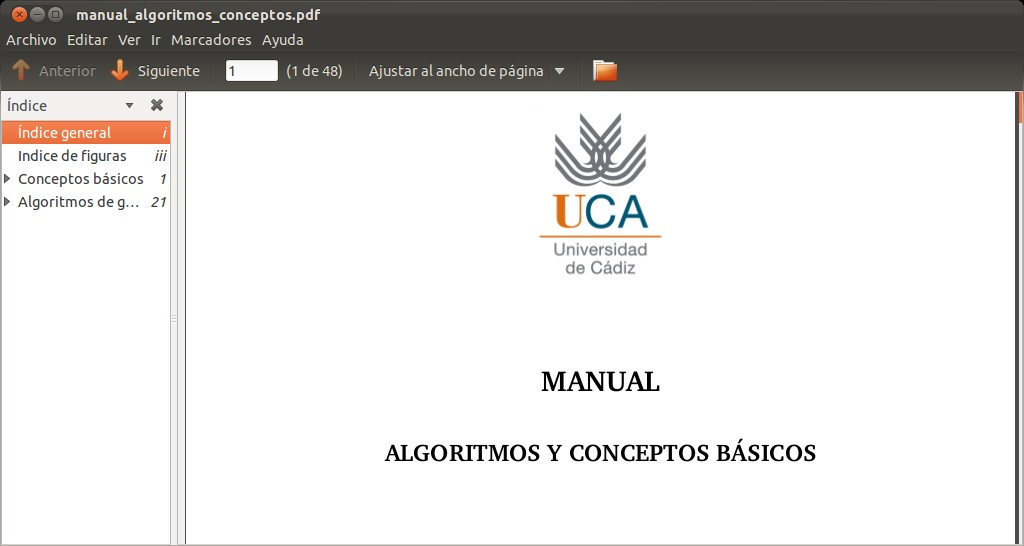
\includegraphics[width=17cm]{./imagenes_documentacion/imagen_manual_algoritmos.jpeg}
\caption{Ventana donde se encuentran disponibles todos los algoritmos de la suite para lectura.}
\end{center}
\end{figure}


Por último en el menú titulado ``sobre Graphvisualx'', se hace una breve mención sobre el creador del proyecto, el nombre del mismo y para la universidad que ha sido desarrollada la aplicación. Su atajo de teclado es: Ctrl+i. \\

\begin{figure}[H]
\begin{center}

\includegraphics[width=17cm]{./imagenes_documentacion/imagen_sobre_graphvisualx.jpeg}
\caption{Ventana donde se visualiza la información relacionada con Graphvisualx.}
\end{center}
\end{figure}

\subsection{Creación grafo}

Grupo de iconos representativos: \icontext{0.4}{0.7}{./imagenes_documentacion/imagen_creacion_grafo.jpeg} \\

Este grupo de botones permiten la siguiente funcionalidad:

\begin{itemize}
\item Nuevo grafo. \quad \icontext{.4}{.9}{./imagenes_documentacion/nuevo.png}
\item Cargar fichero. \quad \icontext{.4}{.9}{./imagenes_documentacion/cargar.png}
\item Aplicar algoritmo. \quad \icontext{.4}{.9}{./imagenes_documentacion/algoritmos.png}
\end{itemize}

Con el botón de nuevo grafo el sistema abre la edición de un nuevo panel o lienzo para que el usuario edite o cree un grafo según los nodos y aristas que desee. Para el caso de las aristas se empleará un sistema de ponderación (etiquetado de las mismas) que se encuentran dentro del dominio de los números enteros.  \\

Cargar fichero permite al usuario cargar desde el propio sistema de ficheros sobre el que trabaje, la introducción de una estructura de tipo grafo almacenada a tal efecto en formato de texto plano. Previamente debería de haberse guardado usando la opción de ``Guardar grafo inicial'' disponible dentro del menú Archivo. \\

Por último se encuentra la opción de aplicar algoritmo que permitirá al usuario desplegar la funcionalidad de la suite para el grafo que se haya editado o cargado previamente en el sistema. Esta opción se encontrará disponible, única y exclusivamente, cuando el usuario haya realizado una carga exitosa de un fichero con la estructura de grafo o cuando haya aceptado el grafo editado en el lienzo de trabajo. En los demás casos esta opción se encontrará deshabilitada. \\

\subsection{Edición grafo}

Grupo de iconos representativos: \icontext{0.4}{0.7}{./imagenes_documentacion/imagen_edicion_grafo.jpeg} \\

Este grupo de botones permiten la siguiente funcionalidad:

\begin{itemize}
\item Crear nodo. \quad \icontext{.4}{.7}{./imagenes_documentacion/nodo.png}
\item Crear arista. \quad \icontext{.4}{.7}{./imagenes_documentacion/arista.png}
\item Borrar contenido lienzo. \quad \icontext{.4}{.7}{./imagenes_documentacion/eraser.png}
\item Mover nodos. \quad \icontext{.4}{.7}{./imagenes_documentacion/mover.png}
\item Aceptar grafo. \quad \icontext{.4}{.7}{./imagenes_documentacion/aceptar.png}
\end{itemize}

Crear nodo permite al usuario la edición de los nodos que desee, en el lienzo de trabajo del grafo dispuesto justo abajo del grupo de botones. Al hacer clic izquierdo se creará un nodo etiquetado según haya o no alguno ya anterior en el lienzo. Por defecto el primer nodo será $0$ y así sucesivamente $0,\ 1,\ 2,\ 3,\ \ldots,\ n$ donde $n \in \mathbb{N}$. Por el contrario al realizar clic derecho sobre un nodo \textbf{previamente creado} en el lienzo de trabajo, este se eliminará de la estructura interna y los demás nodos serán re-etiquetados en respectivo orden. \\

\begin{figure}[H]
\begin{center}
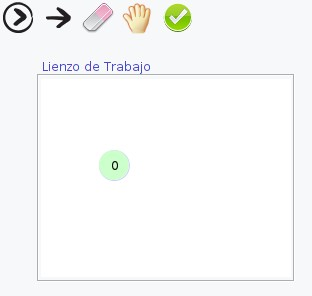
\includegraphics[width=10cm]{./imagenes_documentacion/imagen_nodo_creado_lienzo.jpeg}
\caption{Resultado de hacer clic izquierdo sobre el lienzo una vez se ha seleccionado la opción de crear nodo.}
\end{center}
\end{figure}

Crear arista permite al usuario la edición, sobre los nodos origen y destino que desee, de una arista en el lienzo de trabajo del grafo dispuesto justo abajo del grupo de botones. Es importante tomar constancia que la arista se creará si se realiza un primer clic izquierdo sobre un nodo y posteriormente arrastramos el puntero del ratón hasta soltarlo dentro de otro nodo destino, en caso contrario no sucederá ningún evento asociado. Una vez hayamos hecho clic y luego arrastrado la arista hasta otro nodo, se abrirá una venta emergente en donde podremos introducir el valor asociado a la arista sea dirigida o no. El rango de valores posibles de pesos dentro de la arista esta encuadrado en el dominio de los números enteros con límite superior de $100$ e inferior de $-100$. \\

\begin{figure}[H]
\begin{center}
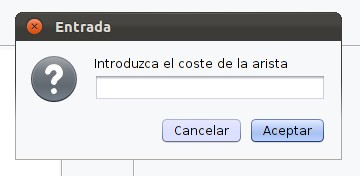
\includegraphics[width=8cm]{./imagenes_documentacion/imagen_valor_arista.jpeg}
\caption{Ventana para introducir el coste de una arista.}
\end{center}
\end{figure}

Una vez que se haya creado la arista podemos realizar estas dos siguientes operaciones si hacemos clic derecho sobre el trozo de la derecha, a partir de la etiqueta, de la arista.

\begin{itemize}
\item Borrar arista. 
\item Modificar coste.
\end{itemize}
 
\begin{figure}[H]
\begin{center}
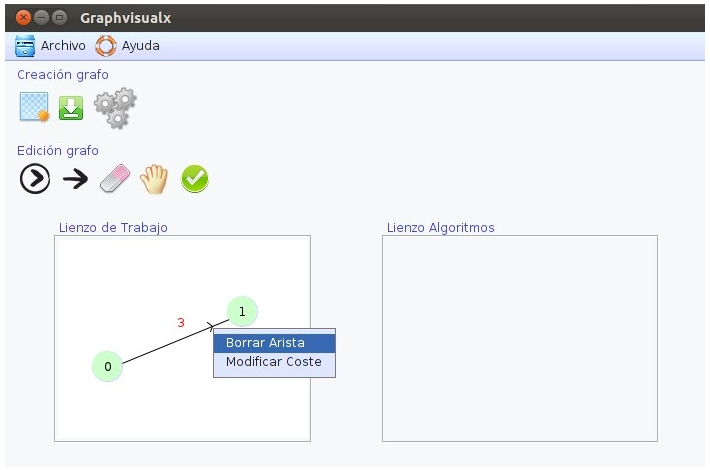
\includegraphics[width=15cm]{./imagenes_documentacion/imagen_nodos_con_arista_opcion_arista_modificada.jpeg}
\caption{Resultado al hacer clic derecho sobre la arista.}
\end{center}
\end{figure}

Borrar arista, como su nombre indica, elimina la arista que une los nodos origen y destino visualmente además de manera interna en la estructura.\\

Modificar coste permite al usuario rectificar un valor asociado al peso o etiquetado de la arista. \\

\newpage

\begin{figure}[H]
\begin{center}
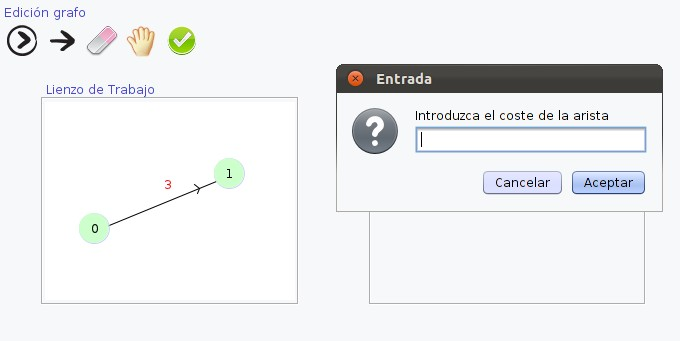
\includegraphics[width=17cm]{./imagenes_documentacion/imagen_icono_modificar_arista.jpeg}
\caption{Resultado de seleccionar la opción de modificar arista en el menú emergente.}
\end{center}
\end{figure}

\subsection{Propiedades del grafo}

Todos los grafos que se pueden tanto editar como cargar en el sistema tienen una serie de propiedades innatas en el cuerpo matemático de los grafos, tales como linealidad, completitud, sentido de la navegabilidad, adyacencia, etc. Dichas propiedades serán visibles para cada grafo (lienzo donde se muestre el grafo tanto inicial como resultado) al realizar la operación de aceptado del grafo tanto en el lienzo de trabajo como al aplicar cualquiera de los algoritmos disponibles del sistema. \\

\begin{figure}[H]
\begin{center}
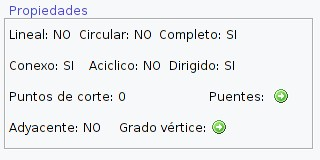
\includegraphics[width=10cm]{./imagenes_documentacion/imagen_propiedades_grafo.jpeg}
\caption{Bloque de contenidos situado abajo de los lienzos donde se visualizan las propiedades de los grafos.}
\end{center}
\end{figure}

Dentro de las propiedades del grafo se encuentran disponibles dos botones: uno tendrá la funcionalidad de hallar el grado del vértice que el usuario desee introduciendo dicho vértice en la ventana emergente a tal efecto y luego hay otro donde permitirá al usuario visualizar, si fuera el caso, los puentes que posee dicho grafo editado en el lienzo de trabajo o cargado en el sistema a través de un fichero. El resultado al pulsar el botón de puentes será visualizado en el lienzo resultado de grafos. \\

\begin{figure}[H]
\begin{center}
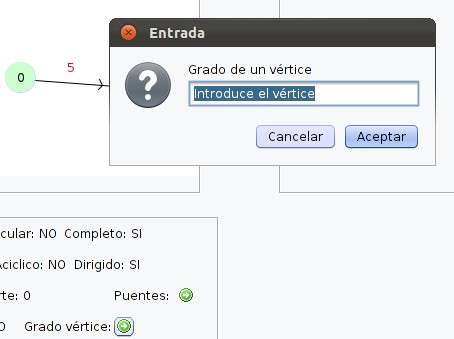
\includegraphics[width=10cm]{./imagenes_documentacion/imagen_grado_vertice_grafo.jpeg}
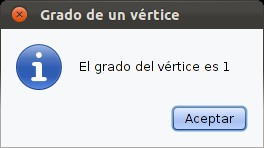
\includegraphics[width=6cm]{./imagenes_documentacion/imagen_grado_grafo_ventana.jpeg}
\caption{Ventana emergente al seleccionar el botón de grado del vértice para el grafo del lienzo.}
\end{center}
\end{figure}

\newpage
\subsection{Algoritmos de grafos}

Finalmente llegamos a la parte principal de la aplicación y así como de procesamiento de los grafo en el sistema. A continuación se muestra una primera captura de la ventana en donde se encuentran establecidos los distintos algoritmos del sistema. 

\begin{figure}[H]
\begin{center}
\hspace*{-.25in}{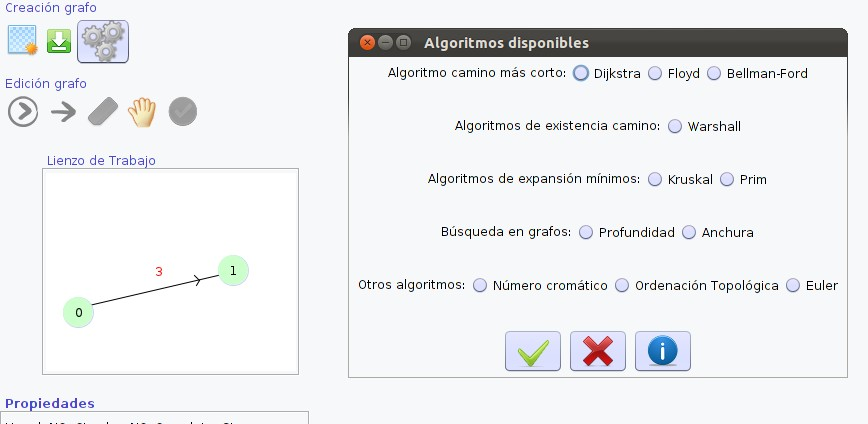
\includegraphics[width=17cm]{./imagenes_documentacion/imagen_icono_algoritmos_ventana_resultante.jpeg}}
\caption{Vista general de la ventana de aplicación de algoritmos sobre el grafo creado.}
\end{center}
\end{figure}

El primer algoritmo disponible, para el procesamiento del camino más corto, es el de Dijkstra \ref{sec:dijkstra}.
\newpage
\begin{figure}[H]
\begin{center}
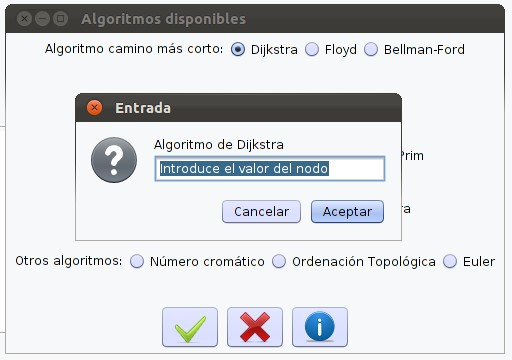
\includegraphics[width=10cm]{./imagenes_documentacion/imagen_icono_dijkstra_ventana_datos.jpeg}
\caption{Ventana emergente de la primera interacción con el algoritmo de Dijkstra.}
\vspace*{.2in}{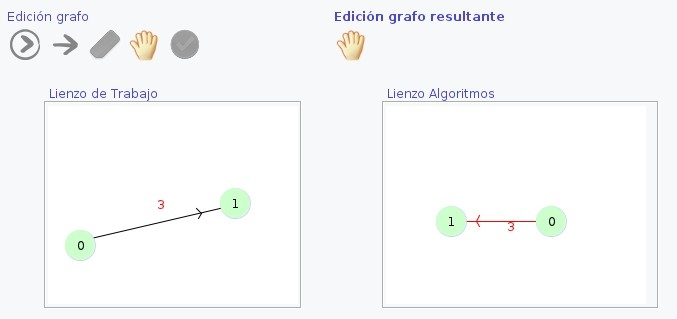
\includegraphics[width=16cm]{./imagenes_documentacion/imagen_resultado_dijkstra_vertice_0.jpeg}}
\caption{Resultado en el lienzo resultado al aplicar sobre el grafo inicial el algoritmo de Dijkstra.}
\end{center}
\end{figure}

\newpage
El segundo algoritmo, también empleado para el procesamiento del camino más corto, es el de Floyd \ref{sec:floyd}.

\begin{figure}[H]
\begin{center}
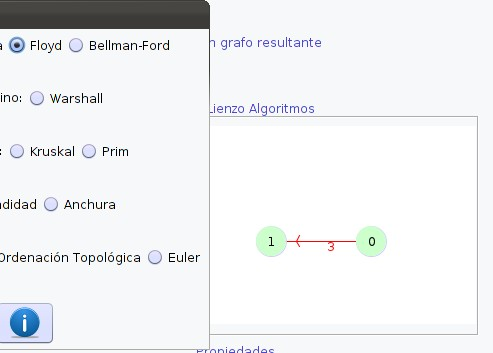
\includegraphics[width=10cm]{./imagenes_documentacion/imagen_resultado_floyd.jpeg}
\caption{Resultado en el lienzo resultado al aplicar sobre el grafo inicial el algoritmo de Floyd.}
\end{center}
\end{figure}

El tercer algoritmo, también empleado para el procesamiento del camino más corto, es el de Bellman-Ford \ref{sec:bellman}. Este algoritmo tiene la peculiaridad de que la ponderación de sus aristas pueden ser de coste tanto negativo como positivo, dentro del domino de los números enteros. Además la suma de los flujos o pesos desde el vértice origen hasta el nodo destino se irán mostrando como pesos asociados al camino posible desde el nodo origen establecido.
\newpage
\begin{figure}[H]
\begin{center}
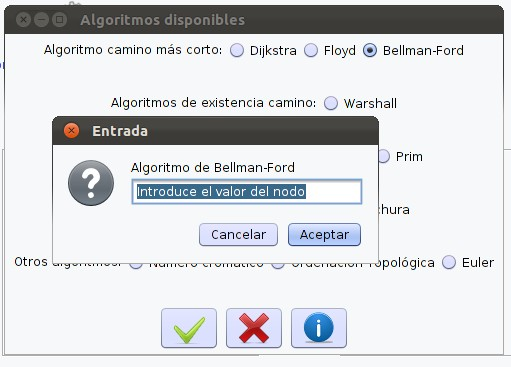
\includegraphics[width=11cm]{./imagenes_documentacion/imagen_bellman_ford_ventana_datos.jpeg}
\caption{Ventana emergente de la primera interacción con el algoritmo de Bellman-Ford.}
\end{center}
\end{figure}

\begin{figure}[H]
\begin{center}
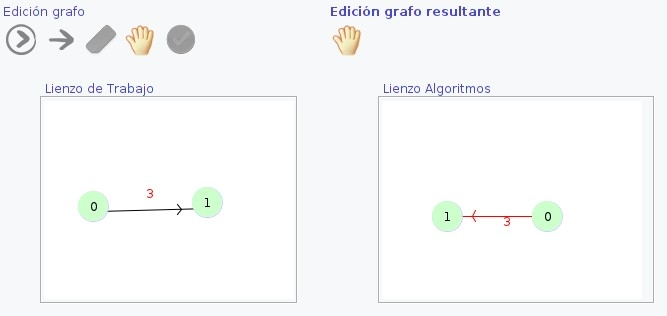
\includegraphics[width=10cm]{./imagenes_documentacion/imagen_resultado_bellman_ford_vertice_0.jpeg}
\caption{Resultado en el lienzo resultado al aplicar sobre el grafo inicial el algoritmo de Bellman-Ford.}
\end{center}
\end{figure}
\newpage
El cuarto algoritmo disponible, que permite averiguar los caminos posibles entre todos los nodos, es Warshall \ref{sec:warshall}.

\begin{figure}[H]
\begin{center}
\includegraphics[width=10cm]{./imagenes_documentacion/imagen_warshall_y_resultado.jpeg}
\caption{Resultado en el lienzo resultado al aplicar sobre el grafo inicial el algoritmo de Warshall.}
\end{center}
\end{figure}

El quinto algoritmo disponible permite obtener el árbol de expansión de coste mínimo para el algoritmo de Kruskal \ref{sec:kruskal}.

\begin{figure}[H]
\begin{center}
\includegraphics[width=10cm]{./imagenes_documentacion/imagen_kruskal_y_resultado.jpeg}
\caption{Resultado en el lienzo resultado al aplicar sobre el grafo el algoritmo de Kruskal.}
\end{center}
\end{figure}
\newpage
El sexto algoritmo disponible permite obtener el árbol de expansión de coste mínimo para el algoritmo de Prim \ref{sec:prim}.

\begin{figure}[H]
\begin{center}
\includegraphics[width=10cm]{./imagenes_documentacion/imagen_prim_y_resultado.jpeg}
\caption{Resultado en el lienzo resultado al aplicar sobre el grafo el algoritmo de Kruskal.}
\end{center}
\end{figure}

El séptimo algoritmo disponible permite el recorrido en anchura del grafo \ref{sec:anchura}.

\begin{figure}[H]
\begin{center}
\includegraphics[width=10cm]{./imagenes_documentacion/imagen_anchura_y_resultado.jpeg}
\caption{Resultado en el lienzo resultado al aplicar sobre el grafo el algoritmo de recorrido en anchura.}
\end{center}
\end{figure}
\newpage
El octavo algoritmo disponible permite el recorrido en profundidad del grafo \ref{sec:profundidad}.

\begin{figure}[H]
\begin{center}
\includegraphics[width=10cm]{./imagenes_documentacion/imagen_profundidad_y_resultado.jpeg}
\caption{Resultado en el lienzo resultado al aplicar sobre el grafo el algoritmo de recorrido en profundidad.}
\end{center}
\end{figure}

El noveno algoritmo disponible permite obtener el número cromático del grafo \ref{sec:cromatico}.

\begin{figure}[H]
\begin{center}
\includegraphics[width=10cm]{./imagenes_documentacion/imagen_numero_cromatico.jpeg}
\caption{Resultado en una ventana emergente donde se dice aproximadamente el número cromático.}
\end{center}
\end{figure}
\newpage
El décimo algoritmo disponible permite obtener la ordenación topológica del grafo \ref{sec:topologico}. El grafo en esta ocasión es distinto al anteriormente usado dado que el anterior al contener una sola arista no mostraba dicha ordenación trivial. \\

\begin{figure}[H]
\begin{center}
\includegraphics[width=13cm]{./imagenes_documentacion/imagen_ordenacion_topologica_y_resultado.jpeg}
\caption{Resultado en el lienzo resultado al aplicar sobre el grafo el algoritmo de Ordenación topológica.}
\end{center}
\end{figure}

Para concluir los algoritmos disponibles tenemos el algoritmo de Euler \ref{sec:euler}.

\begin{figure}[H]
\begin{center}
\includegraphics[width=10cm]{./imagenes_documentacion/imagen_euler.jpeg}
\caption{Resultado en el lienzo resultado al aplicar sobre el grafo el algoritmo de Euler.}
\end{center}
\end{figure}

